\section{Bestiaire}

\subsection{Storm Trooper} \label{sec:storm-trooper}
\begin{figure}[h!]
    \centering
    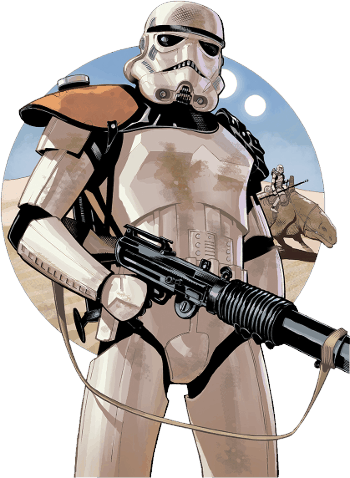
\includegraphics[height=200pt]{_img/dos-au-muur/stormtrooper.png}
\end{figure}
\vspace{-2\baselineskip}
\paragraph{Background}
Soldats dévoués de l’Empire. Certain sont des clones restant de la guerre des clones d’autres non. Ils sont entraînés au combat, équipé d’une bonne armure et armé de Fusil Blaster efficaces.

\paragraph{Traits}

\begin{itemtable}[ c c c c c ]
    \textbf{Agi} & \textbf{Int} & \textbf{\^Ame} & \textbf{For} & \textbf{Vig} \\
    d4           & d6           & d4             & d8           & d8
\end{itemtable}
\begin{itemtable}[ l X ]
    \textbf{Allure}      & 6 \\
    \textbf{Compétences} & Combat d10, Tir d10
\end{itemtable}

\paragraph{Défense}
\begin{itemtable}[ c c ]
    \textbf{Parade}     & \textbf{Résistance} \\
    7                   & 6 (+4)
\end{itemtable}

\paragraph{Attaque}
\begin{itemtable}[ X c c ]
    ~              & \textbf{Combat}   & \textbf{Dégats} \\
    Fusil Blaster  & -                 & 2d8 (3)
\end{itemtable}


\newpage

\subsection{Droïde Combat B1} \label{sec:droide-b1}
\begin{figure}[h!]
    \centering
    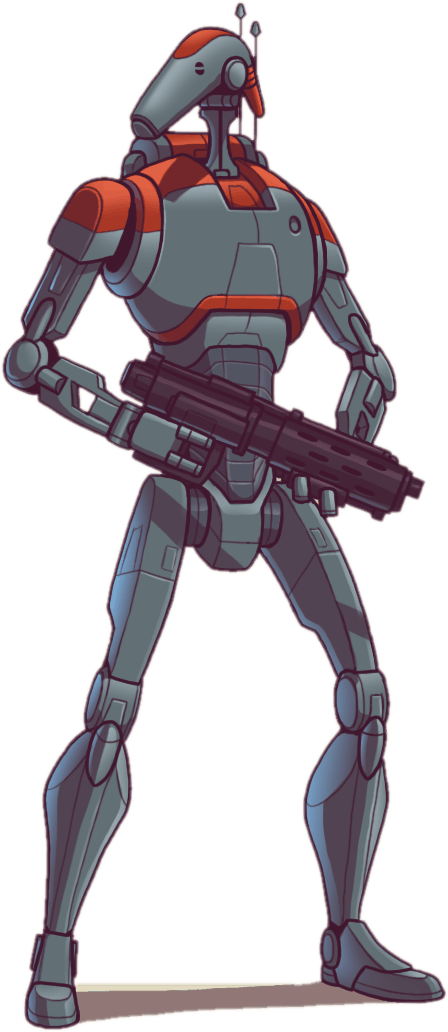
\includegraphics[height=250pt]{_img/songes-de-l-uhumele/droide-b1.png}
\end{figure}
\vspace{-2\baselineskip}
\paragraph{Background}
Bien que ces droïdes ne soient plus produits depuis l’avènement de l’Empire, on en trouve encore quelques bataillons plus ou moins en état sur le marché noir ou au service de gouvernements mineurs et de seigneurs minables de la Bordure Extérieure et de l’Espace Sauvage. Qu’il s’agisse de reliquats des guerres cloniques, de bataillons volés à Baktoid ou tout simplement de troupes assemblées sur une chaîne de montage “récupérée”, les Série N ont continué pendant un certain temps à représenter un produit intéressant pour les acheteurs.

\paragraph{Traits}

\begin{itemtable}[ c c c c c ]
    \textbf{Agi} & \textbf{Int} & \textbf{\^Ame} & \textbf{For} & \textbf{Vig} \\
    d4           & d4           & d4             & d8           & d8
\end{itemtable}
\begin{itemtable}[ l X ]
    \textbf{Allure}      & 6 \\
    \textbf{Compétences} & Combat d8, Tir d10
\end{itemtable}

\paragraph{Défense}
\begin{itemtable}[ c c ]
    \textbf{Parade}     & \textbf{Résistance} \\
    6 (-2)              & 6 
\end{itemtable}

\paragraph{Attaque}
\begin{itemtable}[ X c c ]
    ~              & \textbf{Combat}   & \textbf{Dégats} \\
    Fusil Blaster  & -                 & 2d8 (3)
\end{itemtable}

\newpage

\subsection{Droïdeka} \label{sec:droideka}
\vspace{-4\baselineskip}
\begin{figure}[h!]
    \centering
    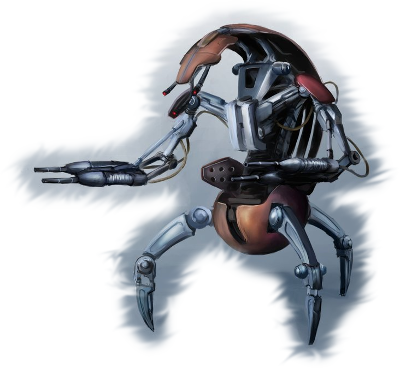
\includegraphics[height=280pt]{_img/songes-de-l-uhumele/droideka.png}
\end{figure}
\vspace{-2\baselineskip}
\paragraph{Background}
Plus connu sous le nom de droïde destroyer, le droïdeka est une redoutable arme. Pour pallier les lacunes des droïdes de combat standards, un appel d’offre fut lancé pour la création d’une arme autrement redoutable. Sur une planète éloignée du c\oe{ur} de la République, une espèce chitineuse nommée les Colicoïdes créa un droïde de combat à sa propre image. Les Colicoïdes sont réputés pour leur insensibilité, et le système de Colla IV a connu maints ennuis, suite à la disparition d’hôtes de passage dévorés. Le droïde destroyer a comblé les attentes des officiers de la Fédération du Commerce, c'est une formidable machine à tuer. 

\paragraph{Traits}

\begin{itemtable}[ c c c c c ]
    \textbf{Agi} & \textbf{Int} & \textbf{\^Ame} & \textbf{For} & \textbf{Vig} \\
    d4           & d4           & d4             & d8           & d8
\end{itemtable}
\begin{itemtable}[ l X ]
    \textbf{Allure}      & 10 \\
    \textbf{Compétences} & Combat d4, Tir d10
\end{itemtable}

\paragraph{Défense / Attaque}
\begin{itemtable}[ X c c ]
    ~                           & \textbf{Parade} & \textbf{Résistance} \\
    ~                           & 4               & 6  \\
    \textbf{Champ déflecteur}   & ~               & +4
\end{itemtable}

\begin{itemtable}[ X c c ]
    ~              & \textbf{Combat}   & \textbf{Dégats} \\
    Canons Blaster & -                 & 2d10 (2)
\end{itemtable}